% TFG - José Ángel Martín Baos. Escuela Superior de Informática. 2018
%%%% CHAPTER: Background %%%
% !TeX spellcheck = en_GB

\chapter{Background}
\label{chap:background}

\drop{T}{his} chapter aims to explain some important concepts used as a basis for the development of this \ac{BSc.} thesis. Firstly, an introduction about Intelligent Transport Systems and traffic modelling is presented. In addition, traffic emissions monitoring and some European measures taken to reduce emissions are discussed. Then, general characteristics of embedded systems are explained and how they can be implemented in traffic and environmental surveillance. It will go on to introduce Raspberry Pi systems and how they can be used in order to achieve the objectives addressed of this \ac{BSc.} Thesis. Finally, H.264/AVC video codec is presented.

\section{Taxonomy of Intelligent Transportation Systems}
\ac{ITS} are tools that combine advanced technologies in communication and information in order to solve transportation problems such as traffic congestion, safety and environmental conservation \cite{San15}. \ac{ITS} can be classified according on their strategic objectives \cite{Rafiq201345} into:
\begin{enumerate}
	\item \emlst{CooperativeMobility.} The development of cooperative systems based on vehicle communications has considerably grown in the last years. These systems require the interconnection of users, vehicles and infrastructure by integrating cooperative applications running on an in-vehicle device.
	
	\item \emlst{EcoMobility.} At the present time, the different modes of transport are essential elements with direct influence on daily life activities. Nonetheless, these transport vehicles are increasing the greenhouse gas emissions with several negative consequences in the environment. For this reason, it is highly important to develop a low carbon economy, so that the environment is threatened as little as possible. EcoMobility pursues this objective by focusing on energy-efficient \ac{ITS}.
	
	\item \emlst{SafeMobility.} Over 40.000 people die on road accidents every year in Europe, which is a significant loss to the society. In addition, these accidents involves a cost of 200 billion euros to the European economy. By the use of \ac{ITS}, the number of accidents on the road can be reduced noticeably. For example, driver assistance systems (ADAS) can be used to detect hazards on the road and to warn drivers about them.
	
	\item \emlst{Infomobility.} In order to develop safer, smarter, and more efficient transport systems, reliable, personalized, and anytime anywhere based real-time travel and traffic information systems are needed. These systems should be aware of the needs, preferences, travel habits, etc. of a particular user.
\end{enumerate}

According with the taxonomy previously reviewed, this project can be classified as EcoMobility, because it pursues to monitor the traffic emissions in urban areas. In \cite{ADASIS,eCo-MOVe, NAVARRO2016314} it can be shown some examples of projects also classified as EcoMobility.

\section{Traffic modelling}
A model is a simplified version of a concept, phenomenon, relationship, structure, system or another aspect of the real world. Therefore, a traffic model is a mathematical model of real world traffic. Traffic models can be classified as \textit{microscopic}, which assumes that the behaviour of an individual vehicle is a function of the traffic conditions in its environment, and \textit{macroscopic}, which assumes an aggregate behaviour of vehicles without considering each individual vehicle. It is assumed that the \ac{ITS} are able to collect the macroscopic magnitudes of \emword{density}, \emword{flow} and \emword{speed} as the essential parameters which characterizes the traffic state and, therefore, the current emission levels derived from the transport.

Density $k$, which is adopted from physics, indicates the number of vehicles per road kilometre. It is calculated as shown in Equation (\ref{eq:4-density}) where ${ \Delta  }_{ X }$ represents a location interval at a specific moment and $n$ is the number of vehicles moving through this interval.
\begin{equation} \label{eq:4-density}
k = \frac { n }{ { \Delta  }_{ X } } 
\end{equation}

The flow rate reflects the number of vehicles that passes a certain cross-section per time unit and it is expressed in vehicles per hour. It is calculated as shown in Equation (\ref{eq:4-flow-rate}), where the variable $m$ represents the number of vehicles passing through a point in a time interval defined by ${ \Delta  }_{ T }$. The maximum capacity of a highway lies between 1800 and 2400 vehicles per hour per traffic lane \cite{HCM2000}.
\begin{equation} \label{eq:4-flow-rate}
q = \frac { m }{ { \Delta  }_{ T } } 
\end{equation}

Finally, the mean speed $u$ is the quotient of the flow rate and the density, as shown in Equation (\ref{eq:4-mean-speed}).
\begin{equation} \label{eq:4-mean-speed}
u = \frac { q }{ k } = \frac{m \cdot {\Delta  }_{ X }}{n \cdot {\Delta  }_{ T }} = \frac { \text{Total  distance  covered  by  vehicles} }{ \text{Total  time  spent  by  vehicles} } 
\end{equation}

\newpage
From the Equation \ref{eq:4-mean-speed} the \emword{fundamental relation} of traffic flow theory can be defined and it is expressed in Equation (\ref{eq:4-fundamental-relation}). Therefore, using this equation the three essentials parameters of a macroscopic traffic model can be reduced to two of them.
\begin{equation} \label{eq:4-fundamental-relation}
q = k \cdot u
\end{equation}

In this project the flow rate is the only parameter measured. Nonetheless, the methodology developed in this project allows to measure the density by locating two consecutive sensors in a road, therefore, a complete traffic model can be generated.


\section{Traffic pollution}
% Introducción general a la problemática, a los sitemas actuales (proyecto europeo). Mencionar los contaminantes a medir. 
% Referencias: (consultar)
%	- Estimación espacio/temporal de la contaminación urbana asociada al tráfico: aplicación a la ciudad de México
%	- Traffic data for local emissions monitoring at a signalized intersection
% 	- Validation of road vehicle and traffic emission models
%	- Modelling instantaneous traffic emission and the influence of traffic speed limits
%	- European project --> https://ec.europa.eu/clima/policies/transport_en
%	- Air quality in Europe — 2016 report

Road transport is often the main source of air pollution in urban areas, for this reason there is an increasing need to estimate precisely its contribution to air pollution on the cities. Therefore, many institutions have developed some emissions models and systems in order to predict the road transport contribution to air pollution. Some systems, such as \ac{DTM} systems can focus on the reduction of emissions, using tools such as variable speed limits, ramp metering, adaptive signal timing \cite{MK10}, vehicle-class routing or prioritization \cite{ZDHB09}. These measures can generate some secondary effects such as longer travel delays, a decrease in the transit performance, or higher greenhouse gas emissions. Therefore, they should only be activated when they are warranted by air quality conditions \cite{EMA09} and reliable emissions models are needed for this purpose. 

The \emword{COPERT} emission model \cite{NS16} can be applied to calculate pollutant emissions due to road traffic. This model is the most commonly used methodology in Europe for the elaboration of official national inventories of emissions due to road traffic \cite{Zaldei2017531}. COPERT model allows to estimate the emissions of six different categories of vehicles. Using this model and the traffic flow rate the levels of the different pollutants can be predicted and, therefore, active traffic control measures on the basis of these estimations can be taken to palliate its effects.

\subsection{Traffic pollution in Europe}
In Europe, transport represents a quarter of its greenhouse gas emissions. Whereas the pollution generated by other sectors has been decreasing during the last years, the transport sector emissions only started to decrease in 2007 and they still remain higher than in 1990, as Figure \ref{fig:4-Emissions-Europe-2016} shows. Consequently, in July 2016, the European Commission adopted a low-emission mobility strategy, which aims to ensure that Europe stays competitive and is able to respond the increasingly mobility needs of people and goods \cite{EuStrat}. 

The \acf{EEA} elaborates annually a report about the Air quality in Europe on the previous years \cite{AirQualityEEA17}. These reports analyse the different effects of air pollution, apart from the sources and emissions of air pollutants. Moreover, the different pollutants and their concentration in Europe are described. In these reports, the \ac{EEA} proposes a maximum concentration for some pollutants such as: PM\textsubscript{10} (small particles of metal, pollen, cement, etc dispersed in the air which diameter is less than 10 µm), PM\textsubscript{2.5}, O\textsubscript{3}, NO\textsubscript{2}, BaP, SO\textsubscript{2}, CO, and other particles.

\begin{figure}[!h]
	\begin{center}
		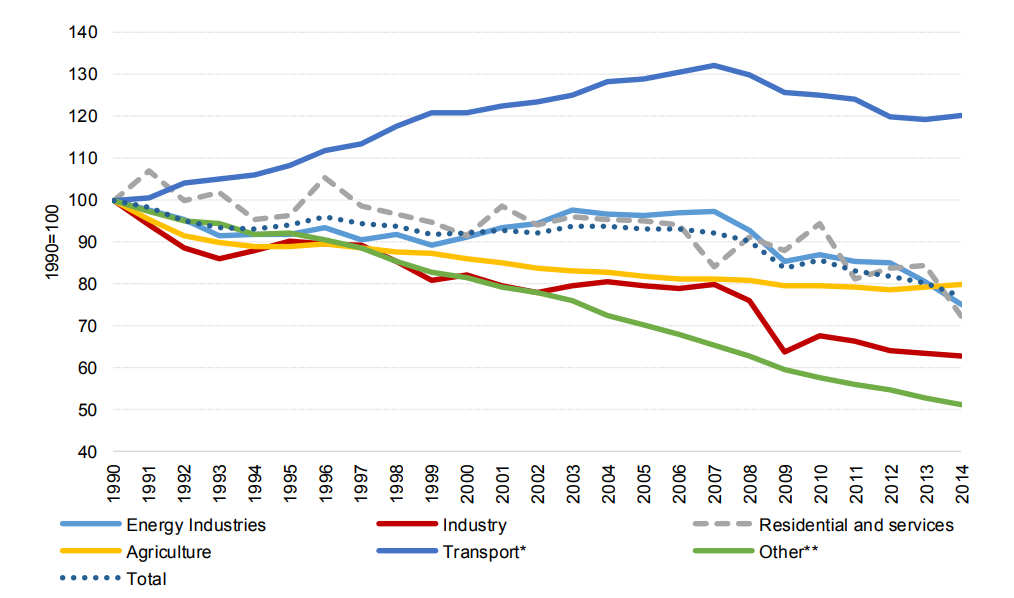
\includegraphics[width=1\textwidth]{4-Emissions-Europe-2016.png}	
		\caption{Evolution of greenhouse gas emissions by sector (1990=100)}{Source: \acf{EEA}}
		\label{fig:4-Emissions-Europe-2016}
	\end{center}
\end{figure}

For the development of this \ac{BSc.} thesis two pollutants are going to be measured: CO and LPG. Carbon monoxide (CO) is one of the main pollutants gases measured for determining the quality of the air. CO is a colourless, odourless, and tasteless toxic gas which makes it very dangerous over certain concentrations. It is generated from the partial oxidation of carbon compounds when there is not enough oxygen to produce carbon dioxide (CO\textsubscript{2}). CO is generated in the exhaust of internal combustion engines or from the incomplete combustion of various fuels, therefore, it can be associated to vehicles, apart form other sources. Liquefied petroleum gas (LPG) is a mixture of hydrocarbon flammable gases such as propane or butane, used as fuel in heating appliances, cooking equipment, and vehicles. It is not considered a pollutant gas by the \ac{EEA}, but actually it can cause air pollution. Hence, it is going to be studied in this work because its presence can be related to fuel leaks in vehicles.

% http://www.airqualitynow.eu/es/about_indices_definition.php
Some projects like \ac{CITEAIR} has been created by the European Union \cite{citeair} in order to develop efficient means to collect, present and compare air quality data across multiple European cities. One of the results of this project was the creation of the \emph{Air quality now} web page \cite{airqualitynow}. This page provides a platform to compare real time air quality measurements on different cities of Europe. In this page, air quality is measured in three different time scales: hourly index during the last day, daily index of the previous day and an annual index. Each of this three time scales has five indices using a pollution scale that goes from 0 (very low) to 100 (very high). Six pollutants are measured: PM\textsubscript{10}, NO\textsubscript{2}, O\textsubscript{3}, CO, PM\textsubscript{2.5}, and SO\textsubscript{2}. Then, the index is calculated depending on the amount of particles per hour (measured in $\mu g/m^3$), except for CO, in which an eight hours moving average is used. Figure \ref{fig:4-Pollution-Index-Airqualitynow} shows the relationship between the pollutant measurement and its pollution index assigned.

\begin{figure}[!h]
	\begin{center}
		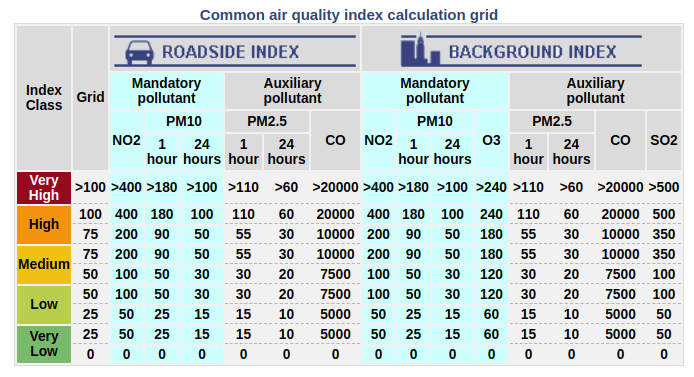
\includegraphics[width=1\textwidth]{4-Pollution-Index-Airqualitynow.png}	
		\caption{Relationship between the pollutant measurement and its assigned pollution index}{Source: Air Quality Now web page \cite{airqualitynow}}
		\label{fig:4-Pollution-Index-Airqualitynow}
	\end{center}
\end{figure}

% Mencionar ciudades como casos de la problemática.
With the goal of evidencing the problem of traffic pollution in big cities, some examples has been selected. Air quality information about Madrid, Berlin and Paris taken on Tuesday 6th of February 2018 are shown in Figure \ref{fig:4-AirQuality-Details}.
As it can be observed, the pollution indices during that day were very high, especially in some cities such as Berlin, where its current roadside pollution level was very high (NO\textsubscript{2} index value is between 75 and 100). Moreover, the previous day (\textit{yesterday} column of the figure) the traffic pollution was even greater, with a NO\textsubscript{2} pollution index over 50 for the three cities. For this reason, some measures should be taken those days, especially in Berlin. This evidence reinforces the fact that some pollution prevention and control mechanisms are necessary.

\begin{figure}[!htbp]
	\centering
	\subfigure[Madrid]{
		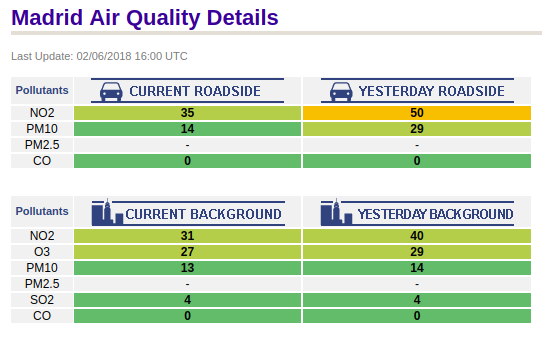
\includegraphics[width=0.74\textwidth]{4-Madrid-AirQuality.png}
		\label{fig:4-Madrid-AirQuality}
	}
	\subfigure[Berlin]{
		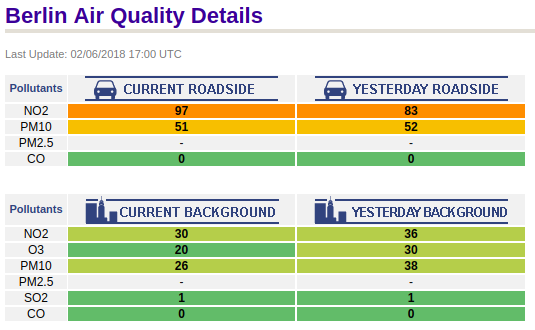
\includegraphics[width=0.74\textwidth]{4-Berlin-AirQuality.png}
		\label{fig:4-Berlin-AirQuality}
	}
	\subfigure[Paris]{
		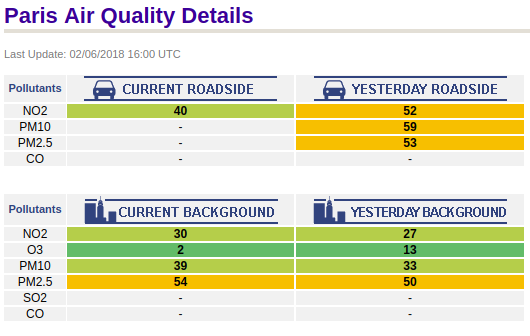
\includegraphics[width=0.74\textwidth]{4-Paris-AirQuality.png}
		\label{fig:4-Paris-AirQuality}
	}
	\caption{Air Quality Details on 6th February 2018 at 18:00}
	\label{fig:4-AirQuality-Details}{Source: Air Quality Now web page \cite{airqualitynow}}
\end{figure}


\newpage
\section{Embedded systems}
% Sistemas Empotrados
An embedded system is an information processing system embedded into enclosing products such as cars, telecommunication or fabrication equipment \cite{Mar16}. Such systems come with some characteristics such as real-time constraints or efficiency requirements. Embedded systems are essential for providing ubiquitous information, which is one of the key goals of modern information technology and \ac{IoT} systems.

Embedded systems are dedicated to specific tasks, therefore computer engineers can optimize them to increase the performance and reliability trying to keep their size, cost, and power consumption as low as possible. Many embedded systems are massively produced benefiting from economies of scales, which make these devices really cheap. For this reason, embedded systems are present in lot of devices, from digital watches, to factory controllers or traffic lights systems. 

% Buscar sistemas embebidos de control de tráfico o medio ambiental.
%	- https://acuraembedded.com/blog/acura-embedded-systems-to-reduce-carbon-emissions-for-public-transport-buses/
%	- ...
% MENCIONAR:
% Estas estaciones solo mide un punto de la ciudad, nosotros buscamos tecnologías baratas y que permitan controlar varios puntos
% Masivo
Embedded systems have been used from early ages to monitor traffic or environmental parameters. Nonetheless, traditionally, these weather and environmental stations (Figure \ref{fig:4-Environmental_Station_Murcia}) were huge and expensive devices that were only placed in the outskirts of big cities. Therefore, the weather information of any location was obtained by interpolating the results of the nearest stations.

\begin{figure}[!h]
	\begin{center}
		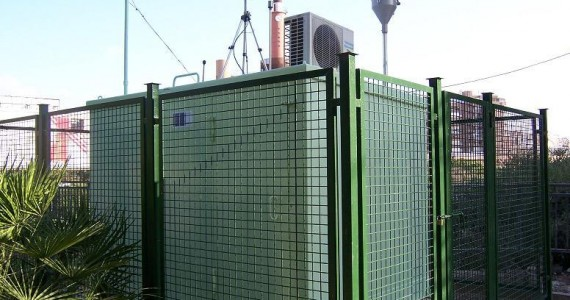
\includegraphics[width=0.9\textwidth]{4-Environmental_Station_Murcia.jpg}
		\caption{Weather station in Murcia}
		\label{fig:4-Environmental_Station_Murcia}{Source: Cartagena IP TV}
	\end{center}
\end{figure}

Nowadays, lots of projects are being developed where modern embedded systems and IoT technologies are used to design weather and pollution monitoring systems. This provides lot of advantages, such as reducing the cost of these systems, or increasing the number of sensors that can be placed in a city (because of the scalability capability of these embedded systems). Taking all these into account, sensors can be located on several points of the city, and consequently, measures would be more accurate. Furthermore, better predictions can be made and, if they are combined with a distributed traffic flow control system, these devices can be used to feed a \ac{DSS} which helps authorities to mitigate environmental problems. In the next paragraphs, some examples of embedded systems used for monitoring environmental parameters are presented.

Acura\footnote{\url{https://acuraembedded.com/blog/acura-embedded-systems-to-reduce-carbon-emissions-for-public-transport-buses}} is an example of an embedded system used to reduce carbon emission in public transport buses. These devices collect the vehicle location, emissions generated and fuel consumed by the buses and send this data to a control center where it is monitored in real-time. The statistics generated are used to reduce the vehicle's carbon footprint.

Bosch Climo\footnote{\url{http://www.boschclimo.com}} is an intelligent air monitoring embedded system designed by Bosch and Intel to evaluate, visualize and act upon the air quality. This solution allows to monitor the ambient air pollutants in real-time thanks to Wi-Fi, GSM, and EDGE network connections. It uses cloud-base analytics of data obtained from lot of sensors to facilitate the energy-efficiency, scalability and sustainability of real-world applications.

% Air Pi
AirPi\footnote{\url{http://airpi.es/}} was a Raspberry Pi shield kit used to monitor temperature, humidity, pressure, light and UV levels, carbon, nitrogen dioxide, and smoke levels. All the information is sent to a web page where it can be visualized. The good point about this kit is the fact that it is very cheap (it costs around 90 dollars).  Nevertheless, this project is no longer available.



\section{Raspberry Pi embedded system}
% Raspberry Pi 3 	-> Evolución
%					-> Comparativa con sus competidores
% 					-> Por qúe se ha elegido?
% !! Muy interesante:  https://www.raspberrypi.org/blog/vectors-from-coarse-motion-estimation/
%					->  Raspbian

A Raspberry Pi \cite{RaspberryPi} is a credit card-sized computer developed originally for education purposes in the United Kingdom by the Raspberry Pi Foundation. This foundation is a charity whose main objective is to promote the power of digital making to people all over the world, especially students. Despite the fact that this device was created to improve programming skills and hardware understanding at the school level, quickly lot of electronics enthusiasts and university researches adopt it for developing projects that require more than a basic microcontroller (for example an Arduino device). Moreover, this microcomputer is capable of doing anything a desktop computer can do, from surfing the web or play high resolution videos, to execute a text processor to edit documents.

The Astro Pi project\footnote{\url{https://astro-pi.org/}} is an example of a project that uses Raspberry Pi devices. This project organized by the \ac{ESA} consists in an annual science and coding competition where students write code for being executed on a Raspberry Pi in the International Space Station.

\subsubsection{Evolution}
% Evolution - Models
First designs from this device are dated in 2006 \cite{Upt11}, nonetheless, the first 50 devices (only for testing) where produced in 2011. During 2012 the first 10,000 Raspberry Pi devices where produced. It is not up to 2014 than the first big update of the device, the \textit{Raspberry Pi 1 B+}, was launched. In 2015 a new version, the \textit{Raspberry Pi 2 B}, was launched, improving the \ac{CPU} and duplicating the RAM memory. That year, the \textit{Raspberry Pi Zero} was also launched, which consisted in a simpler version of the Raspberry Pi 2, but with a cost of 5 Euros. Finally, in the year 2016 the \textit{Raspberry Pi 3 B} was launched, which is the device used in this \ac{BSc.} thesis. This version improves the \ac{CPU} and \ac{GPU} of the previous model maintaining the same cost.  


% Raspberry Pi 3 B
%% Mother board and specs
In the year 2017, when this \ac{BSc.} thesis started, the two latest versions of Raspberry Pi devices where the \textit{Raspberry Pi 3 B} and the \textit{Raspberry Pi Zero W} (an improved version of the \textit{Raspberry Pi Zero} which includes Wi-Fi and Bluetooth connections). The \textit{Raspberry Pi Zero} has a lower size and cost than the rest of the models. Nevertheless, the rest of its specifications are also inferior. Therefore, this device is oriented for industrial applications where very low resources are necessary, whereas the \textit{Raspberry Pi 3 B} is oriented for software applications which requires higher CPU and GPU resources.

The main advantage of the Raspberry Pi device over other alternatives is the fact that it implements a \ac{CPU} and \ac{GPU} on the same motherboard. The processor used in the \textit{Raspberry Pi 3 B} is the Broadcom BCM2837, which is a four cores ARM\footnote{\url{https://www.arm.com/}} 64 bits \ac{CPU}. The ARM processors are used in many \ac{IoT} devices, which makes the Raspberry Pi compatible with lot of the Operating Systems and programs developed for these kinds of devices. Moreover, the four cores allow the execution of several programs that can work concurrently, improving the throughput of the device.

Finally, it is also remarkable that the Raspberry Pi contains a Broadcom VideoCore IV \ac{GPU} which can be used for video compression and motion estimation. This \ac{GPU} allows decoding video with a resolution of 1920x1080 using up to 60 \ac{FPS}. This Broadcom VideoCore \ac{GPU} provides support to all kind of 2D and 3D multimedia applications by the use of OpenGL ES 1.1, OpenGL ES 2.0, hardware-accelerated OpenVG 1.1, Open EGL, OpenMAX, and 1080p30 H.264 high-profile decoder \cite{VideoCoreIV}.


\subsubsection{Alternatives}
% Arduino
There are a great number of devices whose features are similar to the ones of the Raspberry Pi device. In the last years lot of alternatives have been created, such as the \textit{Asus Tinker Board} \cite{Tinker}, the \textit{Banana Pi M64} \cite{M64}, the \textit{OrangePi Plus 2} \cite{OrangePi}, and many more. Nevertheless, the most important alternative is the \textit{Arduino} board \cite{Arduino}. Raspberry Pi and Arduino offers different technical specifications. Table \ref{tab:raspberry-vs-arduino} compares the \textit{Raspberry Pi 3 B} and \textit{Arduino UNO WiFi} devices. In this project, Raspberry Pi has been selected because it offers more adequate technical specifications than Arduino. For example, a relevant factor is the lack of \ac{GPU} in the Arduino, as it is used for the real-time video analysis.

\begin{table}[!h]
	\centering
	{\small
		\begin{tabular}{ |p{.25\textwidth} p{.3\textwidth} p{.3\textwidth}|}
	\hline
	\rowcolor{tabheadbg}
	 & \textscale{.8}{\textbf{Raspberry Pi 3 B}} & \textscale{.8}{\textbf{Arduino UNO WiFi}} \\
	\hline
	\textbf{\ac{CPU}}				& Broadcom BCM2837 & ATmega328 \\
	\hline
	\textbf{\ac{CPU} architecture}	& Quad Core ARM 64bit & Atmel AVR 8-bit \\
	\hline
	\textbf{\ac{CPU} frecuency}		& 1.2 GHz & 2 KB \\
	\hline
	\textbf{\ac{GPU}}				& Broadcom VideoCore IV & No GPU \\
	\hline
	\textbf{Memory}					& 1 GB & 2 KB \\
	\hline
	\textbf{Voltage}				& 5 V & 5 V \\
	\hline
	\textbf{Connections}			& WiFi 2.4GHz 802.11n  & WiFi 802.11 b \\
	 								& 40-pin extended GPIO & 20 Digital I/O Pins \\
	 								& HDMI, CSI and DSI ports & 6 Analog I/O Pins \\ 
									& Ethernet & 6 \acs{PWM} Output Pins \\
									& Bluetooth 4.1 & \\
	\hline
	
\end{tabular}

	}
	\caption{Specifications of \textit{Raspberry Pi 3 B} vs. \textit{Arduino UNO}}
	\label{tab:raspberry-vs-arduino}
\end{table}


\section{Video format H.264/AVC}
\label{subsect:H.264}
Any video is composed by a sequence of images that are reproduced in a sequential way. In H.264/AVC video format and some other video standards each of these video images (or frames) can be classified into three types: I-Frame, P-Frame, and B-Frame \cite{SC11}. Each of this frame types takes advantage of different type of spatial or temporal redundancy of the video sequence: 
\begin{itemize}
	\item \textbf{I-Frame (Inter-frame).} The frame is encoded using only spatial redundancy inside the frame itself.
	\item \textbf{P-Frame (Predictive-frame).} The frame is encoded using as reference a previous I- or P- frame (temporal redundancy).
	\item \textbf{B-Frame (Bi-Predictive-frame).} The frame is encoded using more than one reference image (previous and past frames).
	\item \textbf{Other types}. The extended format of the H.264/AVC decoder support more complex types: SP (Switching P-frame) and SI (Switching I-frame).
\end{itemize}

\subsection{Macroblocks}
\label{subsect:Macroblocks}
A \emword{macroblock} is the basic unit in the video compression formats based on linear block transforms. It contains the information of a 16x16 pixels region of the frame. These blocks contains information about the luminance, the chrominance and the \emword{motion vectors} associated to them. Each macroblock can be divided into several blocks of lower size called partitions \cite{Gir14}, which varies from 16x16 to 4x4, as shown in Figure \ref{fig:4-Macroblocks}. In this figure, it is shown how a macroblock can be divided into two partitions of 16x8 or 8x16, or just in four partitions of 8x8, and each of this 8x8 partitions can be divided into two partitions of 8x4 or 4x8 or into four partitions of 4x4.

\begin{figure}[!h]
	\begin{center}
		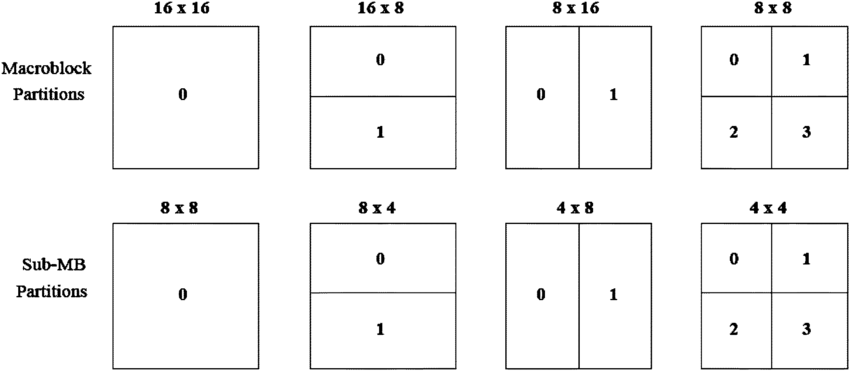
\includegraphics[width=0.8\textwidth]{4-Macroblocks.png}
		\caption{Macroblock partitions}
		\label{fig:4-Macroblocks}
	\end{center}
\end{figure}


\subsection{Motion vectors}
A motion vector represent a temporal redundancy pattern detected between two frames in H.264/AVC and defines a distance and a direction in the form of a bidimensional vector. In other words, they represent the movement of a certain macroblock in the current image with respect to the reference image. Figure \ref{fig:4-Car_with_MV} shows an example of the motion vectors generated by a Raspberry Pi while recording video in a street. Therefore, instead of storing all the pixels for the current frame, the motion vectors corresponding with the macroblocks that have been identified in the reference image are stored, which saves lot of space when storing the video.

PiCamera motion data values for each macroblock are 4-bytes long, as it consists of 1-byte $x$ vector, 1-byte $y$ vector and two 2-byte \ac{SAD} value. If, for example, the resolution of the video is 640x480, there are 41 columns of macroblocks (640 pixels / 16 pixels per macroblock + 1, as PiCamera generates one extra column), and 30 rows (480 pixels / 16 pixels per macroblock). Therefore, each frame generates $41\times30\times4 = 4920$ bytes, which is less than 5KB of motion data. Motion vectors are used in this project to detect the number vehicles that circulates on a street in an interval of time in order to obtain the vehicle flow.

\begin{figure}[!h]
	\begin{center}
		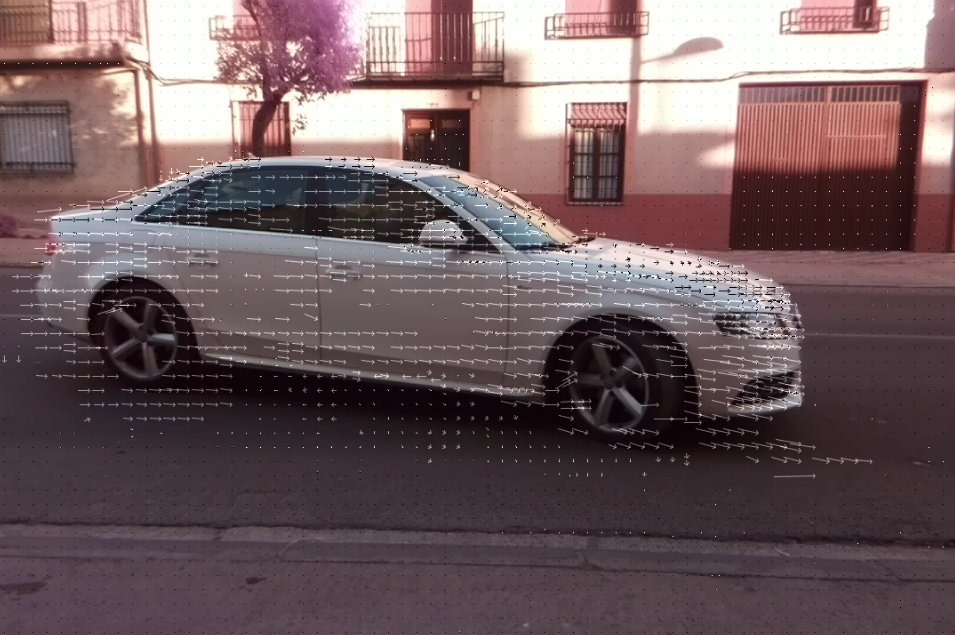
\includegraphics[width=0.8\textwidth]{4-Car_with_MV.png}
		\caption{Example of  the \emword{motion vectors} taken using the developed device}
		\label{fig:4-Car_with_MV}
	\end{center}
\end{figure}

Motion vectors can be represented using their Cartesian coordinates as shown in Equation (\ref{eq:4-mv-cartesian}), where $x$ and $y$ represent the original position of the macroblock in the first frame and $I_{x}$ and $I_{y}$ represent the increments of the vector in each of its coordinates.
\begin{equation} \label{eq:4-mv-cartesian}
mv_{i} = (x, y, I_{x}, I_{y})
\end{equation}

\newpage
Nevertheless, the motion vectors can also be represented usign polar coordinates $r$ and $\theta$ \cite{GRMSJ12}. Therefore, each motion vector can be represented as shown in Equation (\ref{eq:4-mv-polar}).
\begin{equation} \label{eq:4-mv-polar}
mv_{i} = (x, y, r, \theta)
\end{equation} 

Once described the backgorund, in the next chapter the methodology used in this \ac{BSc.} thesis is described.



